\section{Compiler}\label{sec:compiler}
The purpose of a compiler is to convert source code into target code. In the case of the Arc compiler, the source code is text written in the Arc language, and the target code is Arduino language. A generalized model of the compilation process can be see in Figure~\ref{fig:generalcompilermodel}.


\begin{figure}[htb!]
    \centering
    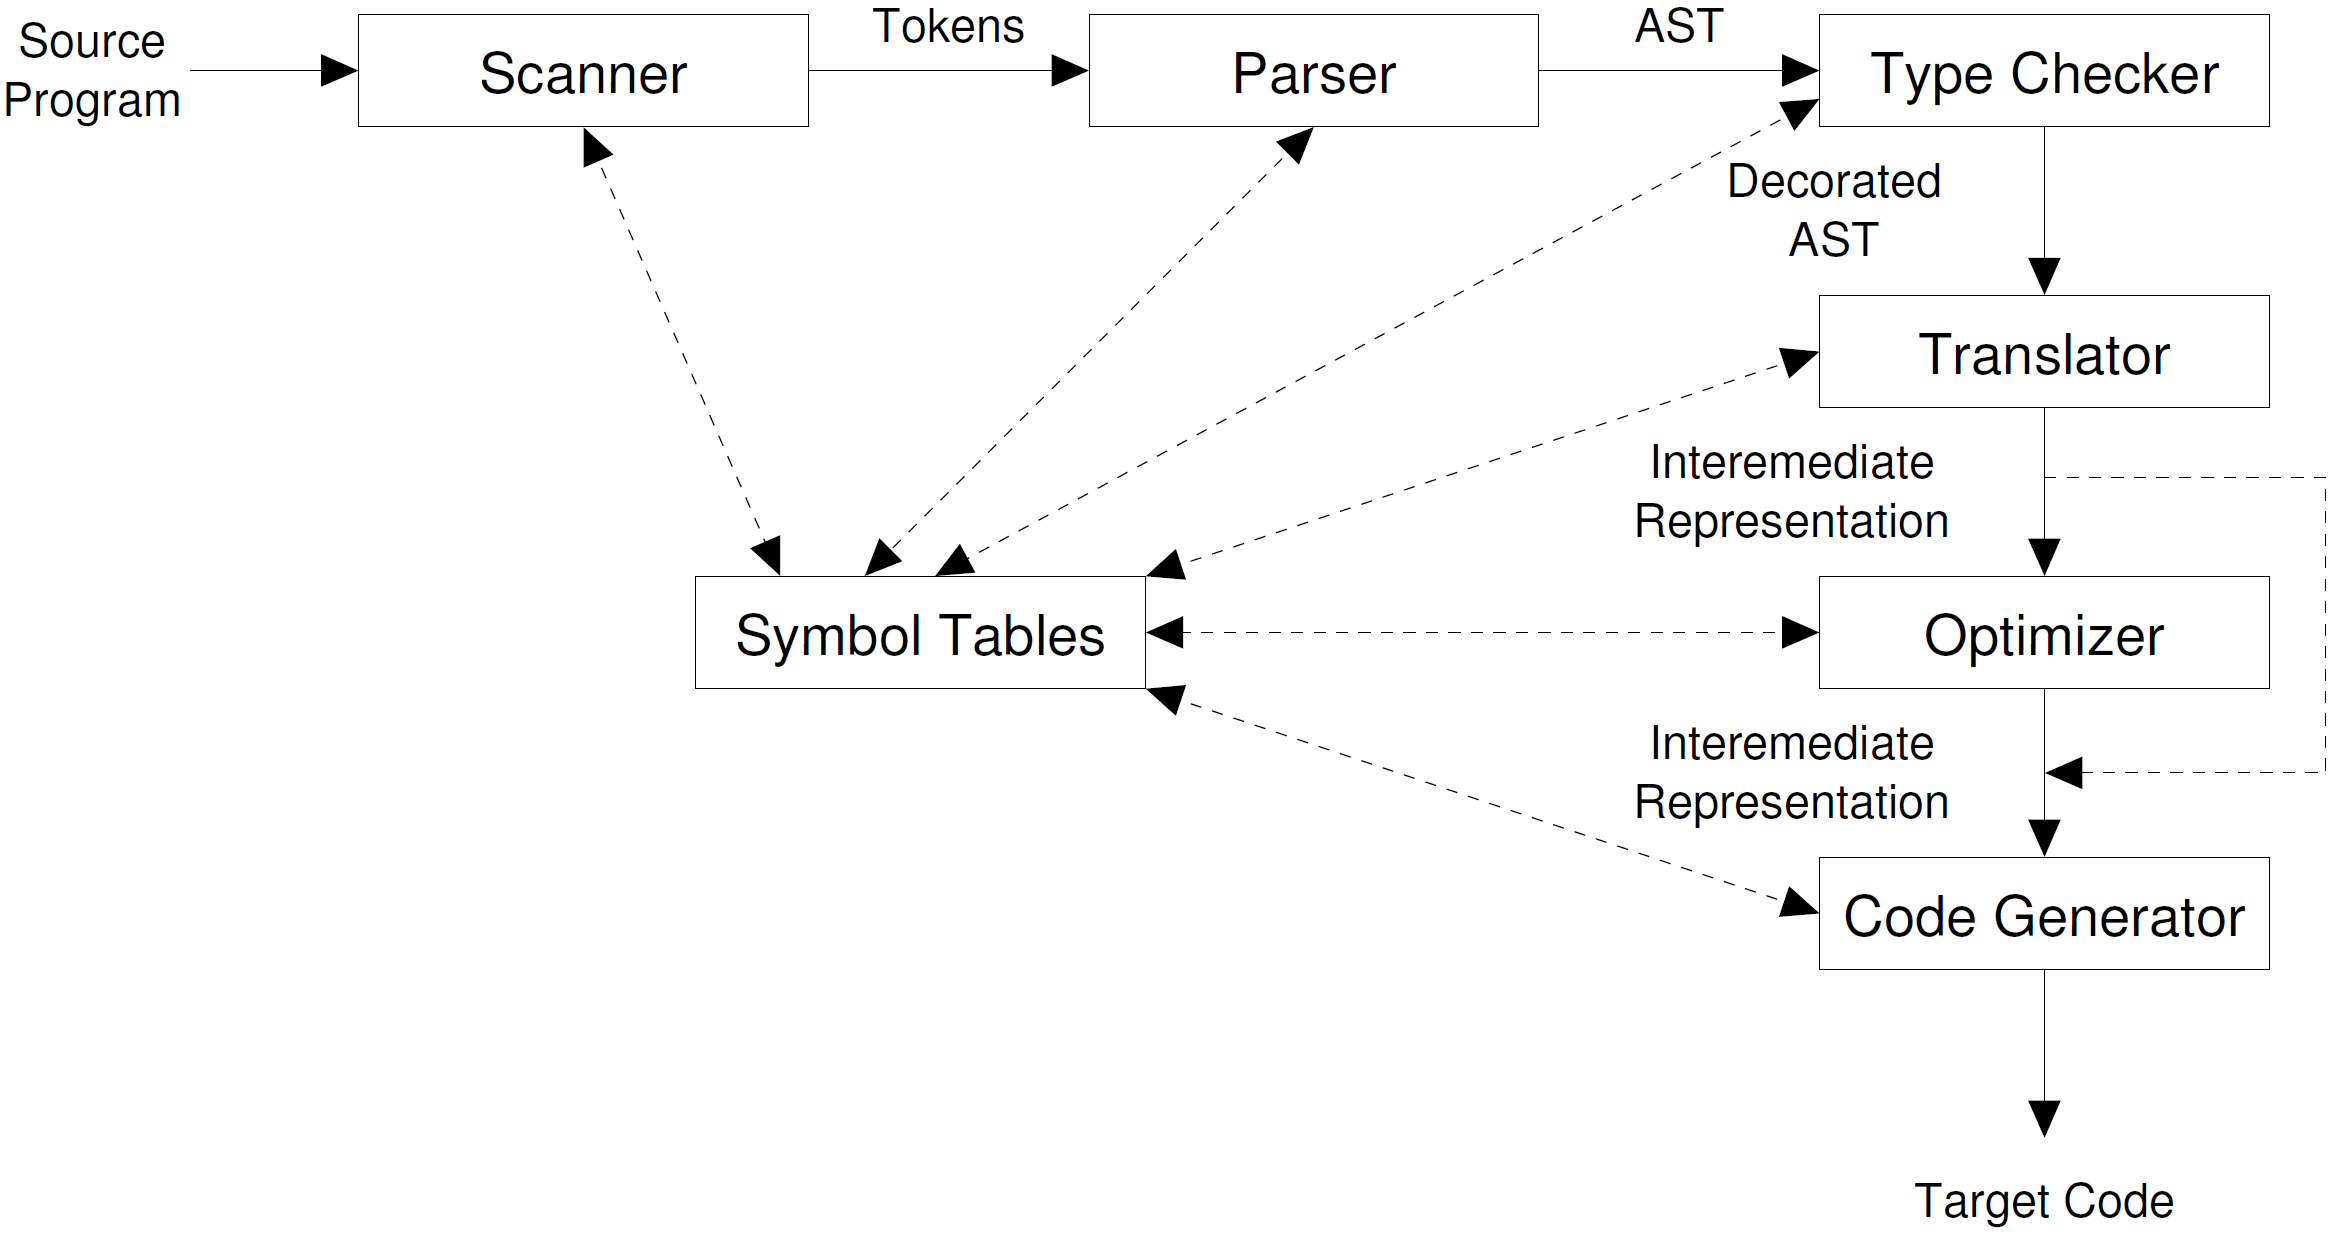
\includegraphics[width=0.8\textwidth]{figures/Full_Compiler.png}
    \caption{A general model of a compiler~\cite{CraftingCompiler}}
    \label{fig:generalcompilermodel}
\end{figure}


The Arc compiler is a bit simpler than the generalized model, and its stages can be seen in Figure~\ref{fig:arccompilermodel}.


\begin{figure}[htb!]
    \centering
    \missingfigure[figwidth=0.8\textwidth]{Insert image of the compilation process for the Arc transpiler}
    %\includegraphics[width=08\textwidth]{}
    \caption{The Arc compiler.}
    \label{fig:arccompilermodel}
\end{figure}


